\section{Results}

Table~\ref{tab:bullying-main-models} presents the M1–M5 estimates for South Africa and Brazil. There is a negative relationship for both Brazil and South Africa between reading scores and bullying penalties. South Africa in Model 1 that just controls for Bullying Penalty indicates a decrease of 55.1 points in reading scores if the learner is bullied on a monthly basis and a decrease of 116.6 points if bullied on a weekly basis. Brazil displays the same negative pattern: learners bullied monthly score 36.4 points lower, while those bullied weekly score 123.5 points lower. All four M1 bullying coefficients are statistically significant at the 1\% level.

The model develops in interesting directions as controls are added in M2, M3, M4 and M5. In South Africa, the estimated bullying penalties become progressively smaller as controls are added, with the M5 coefficients indicating a 36.1-point decrease for monthly bullying and an 80.6-point decrease for weekly bullying. Brazil, by contrast, remains comparatively stable: the monthly penalty increases in magnitude from 36.4 points in M1 to 38.4 points in M5, while the weekly penalty decreases from 123.5 to 113.3 points. The standard errors generally decrease as controls are introduced, indicating greater precision. The explained variance increases from 13.4\% to 38.0\% in South Africa and from 13.9\% to 35.5\% in Brazil.

\begin{table}[!htbp]
\centering
\caption{Bullying and reading achievement: main model sequence}
\label{tab:bullying-main-models}
\scriptsize
\setlength{\tabcolsep}{2.2pt}
\resizebox{\textwidth}{!}{%
\begin{tabular}{lcccccccccc}
\toprule
 & \multicolumn{5}{c}{South Africa} & \multicolumn{5}{c}{Brazil} \\
\cmidrule(lr){2-6}\cmidrule(lr){7-11}
 & M1 & M2 & M3 & M4 & M5 & M1 & M2 & M3 & M4 & M5 \\
\midrule
Bullied about monthly & \shortstack{-55.1***\\(6.9)} & \shortstack{-53.8***\\(6.8)} & \shortstack{-46.8***\\(5.9)} & \shortstack{-43.9***\\(5.5)} & \shortstack{-36.1***\\(5.5)} & \shortstack{-36.4***\\(5.7)} & \shortstack{-37.5***\\(5.4)} & \shortstack{-39.3***\\(5.5)} & \shortstack{-36.5***\\(5.3)} & \shortstack{-38.4***\\(5.8)} \\
Bullied about weekly & \shortstack{-116.5***\\(7.8)} & \shortstack{-110.4***\\(7.5)} & \shortstack{-97.9***\\(6.8)} & \shortstack{-94.2***\\(6.7)} & \shortstack{-80.6***\\(6.7)} & \shortstack{-123.5***\\(7.6)} & \shortstack{-119.2***\\(8.0)} & \shortstack{-112.9***\\(7.3)} & \shortstack{-109.4***\\(7.2)} & \shortstack{-113.3***\\(7.9)} \\
Boy &  & \shortstack{-44.4***\\(3.1)} & \shortstack{-43.4***\\(3.5)} & \shortstack{-40.8***\\(3.8)} & \shortstack{-43.1***\\(3.9)} &  & \shortstack{-10.2**\\(5.0)} & \shortstack{-5.4\\(4.6)} & \shortstack{-3.9\\(4.5)} & \shortstack{-4.9\\(4.8)} \\
Age (years) &  & \shortstack{-10.0***\\(3.0)} & \shortstack{-7.6**\\(3.4)} & \shortstack{-6.9**\\(3.4)} & \shortstack{-7.6**\\(3.3)} &  & \shortstack{-24.6***\\(3.9)} & \shortstack{-13.1***\\(4.4)} & \shortstack{-12.6***\\(4.6)} & \shortstack{-12.7**\\(4.8)} \\
Home SES (ASBHSES scale points) &  &  & \shortstack{25.7***\\(2.3)} & \shortstack{24.9***\\(2.4)} & \shortstack{16.8***\\(2.5)} &  &  & \shortstack{26.3***\\(2.0)} & \shortstack{25.7***\\(2.0)} & \shortstack{21.6***\\(1.8)} \\
Home language: almost always test language &  &  &  & \shortstack{7.4\\(8.1)} & \shortstack{-5.5\\(8.1)} &  &  &  & \shortstack{-18.7*\\(10.7)} & \shortstack{-20.8*\\(10.7)} \\
Home language: sometimes test language &  &  &  & \shortstack{46.3***\\(7.4)} & \shortstack{22.4***\\(7.1)} &  &  &  & \shortstack{7.6\\(9.8)} & \shortstack{12.3\\(9.5)} \\
Home language: never test language &  &  &  & \shortstack{-28.0***\\(8.9)} & \shortstack{-40.7***\\(10.6)} &  &  &  & \shortstack{-93.2***\\(19.2)} & \shortstack{-83.3***\\(19.4)} \\
School location: suburban &  &  &  &  & \shortstack{-18.0\\(17.6)} &  &  &  &  & \shortstack{-1.3\\(15.8)} \\
School location: medium city/large town &  &  &  &  & \shortstack{1.9\\(34.0)} &  &  &  &  & \shortstack{-18.6**\\(9.1)} \\
School location: small town/village &  &  &  &  & \shortstack{-45.1**\\(18.8)} &  &  &  &  & \shortstack{-25.3**\\(11.5)} \\
School location: remote rural &  &  &  &  & \shortstack{-55.5***\\(16.5)} &  &  &  &  & \shortstack{-14.4\\(25.3)} \\
Economically disadvantaged: 11 to 25\% &  &  &  &  & \shortstack{-49.4*\\(27.8)} &  &  &  &  & \shortstack{-25.5**\\(10.9)} \\
Economically disadvantaged: 26 to 50\% &  &  &  &  & \shortstack{-82.8***\\(20.2)} &  &  &  &  & \shortstack{-47.6***\\(13.7)} \\
Economically disadvantaged: more than 50\% &  &  &  &  & \shortstack{-117.3***\\(17.1)} &  &  &  &  & \shortstack{-40.9***\\(11.7)} \\
Other gender category &  &  &  &  &  &  & \shortstack{-100.2***\\(31.1)} & \shortstack{-86.7**\\(35.1)} & \shortstack{-85.6**\\(35.6)} & \shortstack{-49.1**\\(23.6)} \\
\midrule
Learners & 11,660 & 11,618 & 9,167 & 8,505 & 7,177 & 4,715 & 4,706 & 4,110 & 4,022 & 3,563 \\
$R^{2}$ & 0.134 & 0.170 & 0.278 & 0.296 & 0.380 & 0.139 & 0.165 & 0.317 & 0.324 & 0.355 \\
\bottomrule
\end{tabular}%
}
\parbox{0.98\textwidth}{\footnotesize \textit{Notes:} Entries are coefficients with jackknife standard errors in parentheses. The reference group is almost never bullied; the gender reference is girls. All models use the default PIRLS student weight and all five reading plausible values. M1 includes bullying; M2 adds gender and age; M3 adds continuous home SES; M4 adds home language; M5 adds school location and economically disadvantaged composition. Significance: *** p\textless{}0.01, ** p\textless{}0.05, * p\textless{}0.10.}
\end{table}

\FloatBarrier

Figure~\ref{fig:bullying-coefficients} summarizes the bullying coefficients across M1–M5, showing how the estimated associations change as successive controls are introduced.
\begin{figure}[!htbp]
\centering
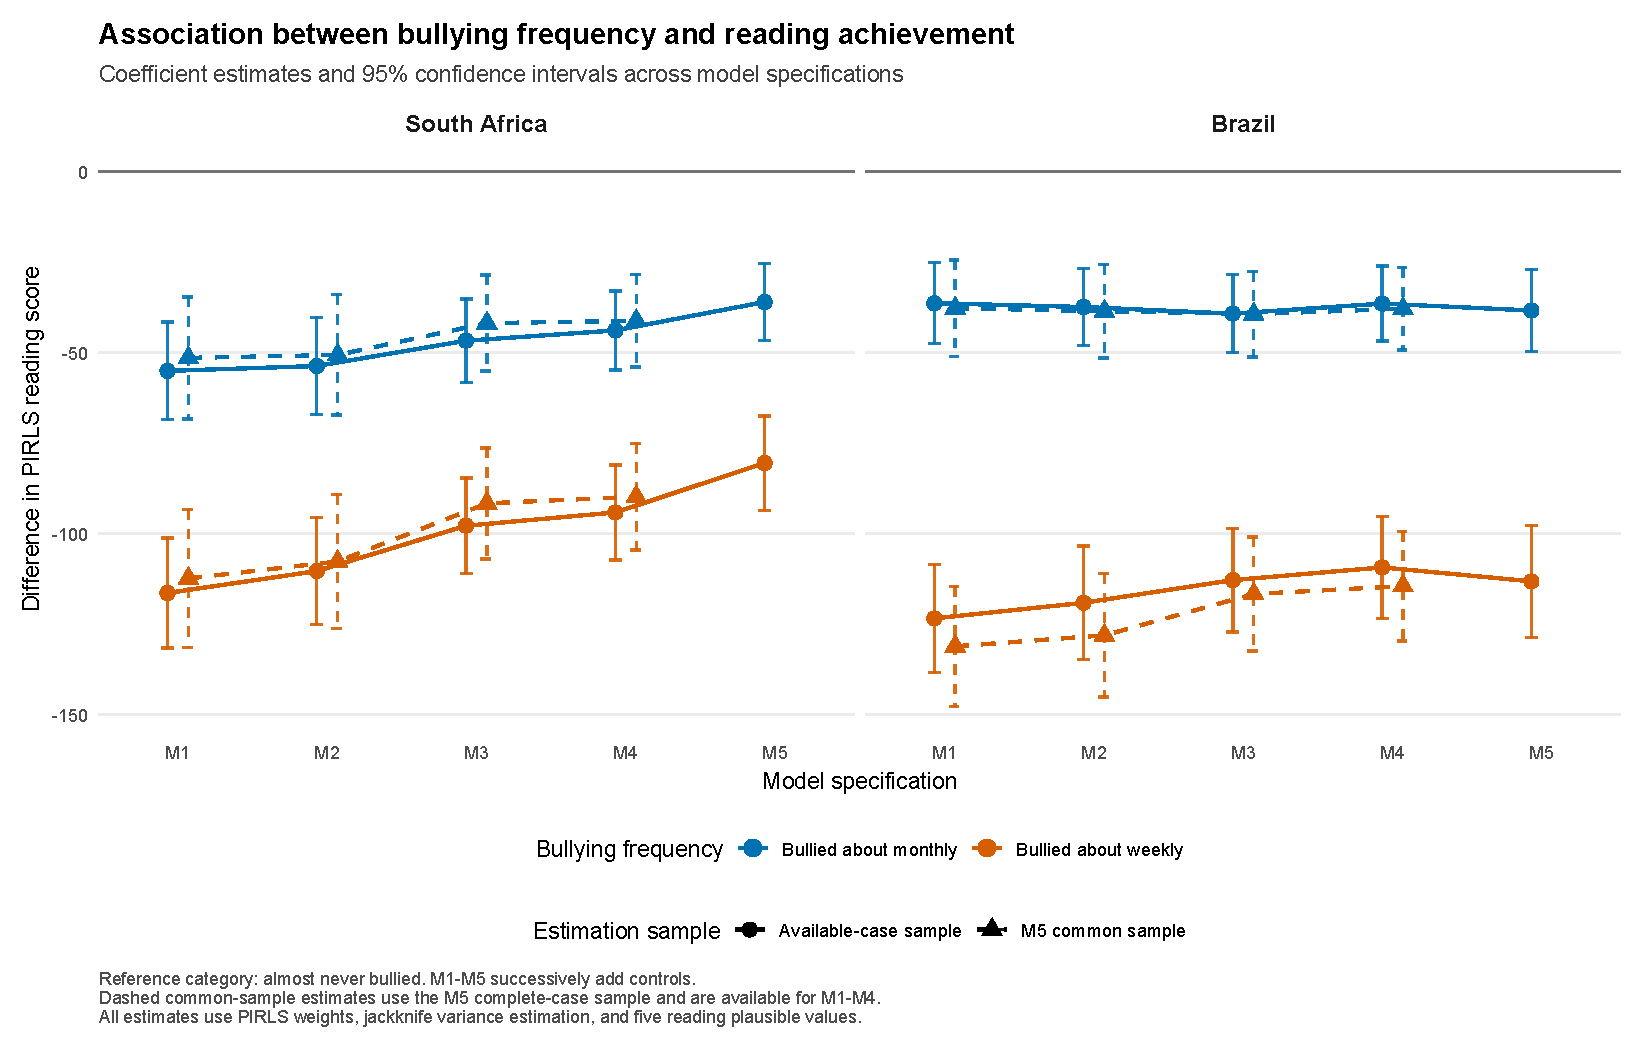
\includegraphics[width=\textwidth]{../../output/regressions/figures/bullying_coefficients_across_models.pdf}
\caption{Estimated association between bullying frequency and reading achievement across model specifications}
\label{fig:bullying-coefficients}
\end{figure}
\FloatBarrier

Re-estimating M1–M4 on the common M5 sample produced a similar pattern of coefficients, suggesting that the changes across models were not primarily attributable to sample composition (Appendix Table~\ref{tab:bullying-common-sample}). The continuous-scale specification also produced results consistent with the main analysis (Appendix Table~\ref{tab:bullying-robustness}).

Table~\ref{tab:bullying-interactions} presents the interactions between bullying and gender (I1) and between bullying and home SES (I2). The gender interactions are not statistically significant in either South Africa or Brazil. There is therefore no evidence that the association between bullying and reading achievement differs between boys and girls.

The SES interaction produces a different pattern. In South Africa, each one-unit increase in home SES makes the estimated monthly bullying penalty 13.2 points more negative and the weekly penalty 20.3 points more negative. In Brazil, the corresponding interaction coefficients are positive: 3.2 points for monthly bullying and 9.0 points for weekly bullying. The monthly interaction is not statistically significant, whereas the weekly interaction is significant at the 5\% level. Thus, there is evidence that higher SES intensifies the bullying penalty in South Africa, while the Brazilian estimates provide limited evidence that higher SES moderates the weekly bullying penalty.

\begin{table}[!htbp]
\centering
\caption{Heterogeneity in the association between bullying and reading achievement}
\label{tab:bullying-interactions}
\scriptsize
\setlength{\tabcolsep}{2.2pt}
\resizebox{\textwidth}{!}{%
\begin{tabular}{lcccc}
\toprule
 & \multicolumn{2}{c}{South Africa} & \multicolumn{2}{c}{Brazil} \\
\cmidrule(lr){2-3}\cmidrule(lr){4-5}
 & I1 & I2 & I1 & I2 \\
\midrule
Bullied about monthly & \shortstack{-46.5***\\(7.0)} & \shortstack{-42.2***\\(5.7)} & \shortstack{-34.1***\\(8.8)} & \shortstack{-39.8***\\(5.6)} \\
Bullied about weekly & \shortstack{-95.3***\\(7.8)} & \shortstack{-95.5***\\(6.4)} & \shortstack{-120.4***\\(10.6)} & \shortstack{-110.9***\\(6.9)} \\
Boy & \shortstack{-41.2***\\(6.7)} & \shortstack{-42.9***\\(3.4)} & \shortstack{-4.1\\(4.9)} & \shortstack{-5.6\\(4.7)} \\
Age (years) & \shortstack{-7.6**\\(3.4)} & \shortstack{-8.0**\\(3.4)} & \shortstack{-12.9***\\(4.4)} & \shortstack{-13.5***\\(4.3)} \\
Home SES (ASBHSES scale points) & \shortstack{25.7***\\(2.3)} &  & \shortstack{26.2***\\(2.1)} &  \\
Bullied about monthly × Boy & \shortstack{-0.7\\(9.4)} &  & \shortstack{-10.5\\(11.1)} &  \\
Bullied about weekly × Boy & \shortstack{-5.1\\(7.4)} &  & \shortstack{9.9\\(12.7)} &  \\
Home SES (centred scale points) &  & \shortstack{37.5***\\(2.8)} &  & \shortstack{24.1***\\(2.0)} \\
Bullied about monthly × Home SES (centred scale points) &  & \shortstack{-13.2***\\(2.8)} &  & \shortstack{3.2\\(3.0)} \\
Bullied about weekly × Home SES (centred scale points) &  & \shortstack{-20.3***\\(2.8)} &  & \shortstack{9.0**\\(4.5)} \\
Other gender category &  &  &  & \shortstack{-86.7**\\(35.2)} \\
\midrule
Learners & 9,167 & 9,167 & 4,076 & 4,110 \\
$R^{2}$ & 0.278 & 0.289 & 0.314 & 0.319 \\
\bottomrule
\end{tabular}%
}
\parbox{0.98\textwidth}{\footnotesize \textit{Notes:} Entries are coefficients with jackknife standard errors in parentheses. I1 interacts bullying with gender and excludes Brazil's 41 learners in the Other gender category. I2 interacts bullying with continuous ASBHSES centred at the design-weighted country mean; one unit is one PIRLS ASBHSES scale point. The reference bullying category is almost never and the gender reference is girls. Significance: *** p\textless{}0.01, ** p\textless{}0.05, * p\textless{}0.10.}
\end{table}

\FloatBarrier
